% Options for packages loaded elsewhere
\PassOptionsToPackage{unicode}{hyperref}
\PassOptionsToPackage{hyphens}{url}
%
\documentclass[
  12pt,
]{article}
\usepackage{lmodern}
\usepackage{amssymb,amsmath}
\usepackage{ifxetex,ifluatex}
\ifnum 0\ifxetex 1\fi\ifluatex 1\fi=0 % if pdftex
  \usepackage[T1]{fontenc}
  \usepackage[utf8]{inputenc}
  \usepackage{textcomp} % provide euro and other symbols
\else % if luatex or xetex
  \usepackage{unicode-math}
  \defaultfontfeatures{Scale=MatchLowercase}
  \defaultfontfeatures[\rmfamily]{Ligatures=TeX,Scale=1}
\fi
% Use upquote if available, for straight quotes in verbatim environments
\IfFileExists{upquote.sty}{\usepackage{upquote}}{}
\IfFileExists{microtype.sty}{% use microtype if available
  \usepackage[]{microtype}
  \UseMicrotypeSet[protrusion]{basicmath} % disable protrusion for tt fonts
}{}
\makeatletter
\@ifundefined{KOMAClassName}{% if non-KOMA class
  \IfFileExists{parskip.sty}{%
    \usepackage{parskip}
  }{% else
    \setlength{\parindent}{0pt}
    \setlength{\parskip}{6pt plus 2pt minus 1pt}}
}{% if KOMA class
  \KOMAoptions{parskip=half}}
\makeatother
\usepackage{xcolor}
\IfFileExists{xurl.sty}{\usepackage{xurl}}{} % add URL line breaks if available
\IfFileExists{bookmark.sty}{\usepackage{bookmark}}{\usepackage{hyperref}}
\hypersetup{
  pdftitle={Policing for Profit and the Undermining of Democracy},
  pdfauthor={Jonathan Ben-Menachem; Kevin Morris},
  hidelinks,
  pdfcreator={LaTeX via pandoc}}
\urlstyle{same} % disable monospaced font for URLs
\usepackage[margin=1in]{geometry}
\usepackage{longtable,booktabs}
% Correct order of tables after \paragraph or \subparagraph
\usepackage{etoolbox}
\makeatletter
\patchcmd\longtable{\par}{\if@noskipsec\mbox{}\fi\par}{}{}
\makeatother
% Allow footnotes in longtable head/foot
\IfFileExists{footnotehyper.sty}{\usepackage{footnotehyper}}{\usepackage{footnote}}
\makesavenoteenv{longtable}
\usepackage{graphicx}
\makeatletter
\def\maxwidth{\ifdim\Gin@nat@width>\linewidth\linewidth\else\Gin@nat@width\fi}
\def\maxheight{\ifdim\Gin@nat@height>\textheight\textheight\else\Gin@nat@height\fi}
\makeatother
% Scale images if necessary, so that they will not overflow the page
% margins by default, and it is still possible to overwrite the defaults
% using explicit options in \includegraphics[width, height, ...]{}
\setkeys{Gin}{width=\maxwidth,height=\maxheight,keepaspectratio}
% Set default figure placement to htbp
\makeatletter
\def\fps@figure{htbp}
\makeatother
\setlength{\emergencystretch}{3em} % prevent overfull lines
\providecommand{\tightlist}{%
  \setlength{\itemsep}{0pt}\setlength{\parskip}{0pt}}
\setcounter{secnumdepth}{5}
\usepackage{rotating}
\usepackage{setspace}
\usepackage{booktabs}
\usepackage{longtable}
\usepackage{array}
\usepackage{multirow}
\usepackage{wrapfig}
\usepackage{float}
\usepackage{colortbl}
\usepackage{pdflscape}
\usepackage{tabu}
\usepackage{threeparttable}
\usepackage{threeparttablex}
\usepackage[normalem]{ulem}
\usepackage{makecell}
\usepackage{xcolor}
\newlength{\cslhangindent}
\setlength{\cslhangindent}{1.5em}
\newenvironment{cslreferences}%
  {\setlength{\parindent}{0pt}%
  \everypar{\setlength{\hangindent}{\cslhangindent}}\ignorespaces}%
  {\par}

\title{Policing for Profit and the Undermining of Democracy\thanks{The authors thank XX for their feedback and support. All errors are our responsibility.}}
\usepackage{etoolbox}
\makeatletter
\providecommand{\subtitle}[1]{% add subtitle to \maketitle
  \apptocmd{\@title}{\par {\large #1 \par}}{}{}
}
\makeatother
\subtitle{Fines, Fees, and Turnout}
\author{Jonathan Ben-Menachem\footnote{PhD Student, Columbia University, Department of Sociology (\href{mailto:jb4487@columbia.edu}{\nolinkurl{jb4487@columbia.edu}})} \and Kevin Morris\footnote{Researcher, Brennan Center for Justice at NYU School of Law (\href{mailto:kevin.morris@nyu.edu}{\nolinkurl{kevin.morris@nyu.edu}})}}
\date{January 27, 2021}

\begin{document}
\maketitle
\begin{abstract}
This is an abstract.
\end{abstract}

\pagenumbering{gobble}
\pagebreak

\pagenumbering{arabic}
\begin{center}
Policing for Profit and the Undermining of Democracy: Fines, Fees, and Turnout \\
Jonathan Ben-Menachem and Kevin Morris
\end{center}

Fines and fees are increasingly recognized as a form of racist revenue extraction connected to marginalized communities' alienation from government. American cities' reliance on fines and fees revenue increased significantly following the 2008 recession --- as local tax revenues dropped and tax increases became less politically viable, jurisdictions increased the amounts of fines and fees and imposed them more frequently in order to fund government services (Singla, Kirschner, and Stone \protect\hyperlink{ref-Singla2020}{2020}; Mughan \protect\hyperlink{ref-Mughan2020}{2020}; Kirk, Fernandes, and Friedman \protect\hyperlink{ref-Kirk2020}{2020}; Martin \protect\hyperlink{ref-Martin2018}{2018}). Although a body of literature developed over the past decade indicates that criminalization chills political participation, no work has directly investigated the relationship between fines and fees revenue collection and voter turnout. This project intends to fill that gap by testing whether fines and fees at the municipal level influence voter turnout.

Fines and fees practices disproportionately target Black Americans: city government reliance on fines and fees revenue is associated with larger Black populations, racial stereotypes affect the imposition of fines and fees, and Black defendants face more severe penalties related to monetary sanctions (United States Commission on Civil Rights \protect\hyperlink{ref-UnitedStatesCommissiononCivilRights2017}{2017}; Harris, Evans, and Beckett \protect\hyperlink{ref-Harris2011}{2011}; Edwards and Harris \protect\hyperlink{ref-Edwards2020}{2020}). The relationship between cities' reliance on fines and fees and the proportion of Black residents is significantly diminished when Black communities are represented by at least one Black legislator, however (Sances and You \protect\hyperlink{ref-Sances2017}{2017}). This could suggest that higher reliance on fines and fees results from government officials targeting individuals who hold less political power (Makowsky and Stratmann \protect\hyperlink{ref-Makowsky2009}{2009}).

Additionally, Sances and You (\protect\hyperlink{ref-Sances2017}{2017}) explicitly suggested that ``fines may make descriptive representation less likely by depressing minority turnout,'' and called for further research regarding voter turnout and the imposition of fines. In this paper, we clarify that relationship by picking up where Sances and You (\protect\hyperlink{ref-Sances2017}{2017}) left off. By tying data from the 2012 and 2017 Census of Governments to a national geocoded voter file we test whether municipalities with more fees and fines collected per resident saw lower turnout in the 2014 and 2018 general elections. We expect to find that municipalities where more revenue is raised per resident saw lower turnout, other things being equal. Because the American criminal legal system falls disproportionately on minorities, we also expect that the racial turnout gap (Fraga \protect\hyperlink{ref-Fraga2018}{2018}) will be larger in municipalities that rely more heavily on fines and fees. Of course, fines and fees imposition may be related to turnout without necessarily indicating a causal relationship. For this reason we leverage data on fines collections and turnout from multiple time periods to investigate the causal relationship.

Fines and fees legally disenfranchise Americans: 48 states and the District of Columbia authorize some form of wealth-based penal disenfranchisement (Colgan \protect\hyperlink{ref-Colgan2019}{2019}). More specifically, many states require payment of fees as a condition of criminal legal supervision or the payment of all legal financial obligations as a condition of completing a sentence, and failure to comply with supervision conditions or sentence completion conditions can be a barrier to voting rights restoration. A recent report from the Sentencing Project estimates that more than 5 million Americans are legally barred from voting due to a felony conviction (Uggen et al. \protect\hyperlink{ref-Uggen2020}{2020}), and the role of fees and fines in the context of felony disenfranchisement has taken on greater significance in the past year. After Floridians voted to restore voting rights to individuals with felony convictions, Florida legislators passed legislation requiring these individuals to pay off the fees and fines associated with their original sentence. Because Florida does not maintain good records on who owes how much, this has proved a major hurdle for would-be voters.

Recent work from scholars in sociology and political science, however, indicates that many more voters are also \emph{indirectly} disenfranchised due to over-incarceration and the politically chilling effects of the carceral state. Policing and incarceration shape political socialization: personal contact with police or incarceration is associated with a reduced likelihood of political participation, and that alienating effect extends even to people who have incarcerated family members or who simply reside in affected communities (Lee, Porter, and Comfort \protect\hyperlink{ref-Lee2014}{2014}; Weaver and Lerman \protect\hyperlink{ref-Weaver2010}{2010}; Morris \protect\hyperlink{ref-Morris2020}{2020}). This relationship is complicated, however. In New York City, concentrated stop-and-frisk activity was associated with \emph{reduced} turnout in Congressional elections, but \emph{increased} turnout in the 2008 presidential election as well as the local mayoral election in 2013 (Laniyonu \protect\hyperlink{ref-Laniyonu2019}{2019}). It may also be the case that proximal contact differs from personal contact with the criminal legal system --- whereas direct experience with criminalization (and incarceration in particular) reduces the likelihood of voting, proximal or indirect experience produces more mixed results. Hannah Walker suggests that police contact that does not lead to a criminal conviction may even mobilize voters --- but her survey questions specifically excluded ``minor traffic stops,'' a primary site of police ticketing (Walker \protect\hyperlink{ref-Walker2014}{2014}).

Despite this burgeoning literature, one of the most routine interactions Americans have with the police has gone largely unstudied: namely, ticketing for low-level offenses. Police ticketing practices may discourage potential voters without directly disenfranchising them, and ticketing affects more Americans than legal disenfranchisement. In 2018, more than 24 million people experienced police contact in the context of a traffic stop; by contrast, about 5.17 million people are disenfranchised as a result of a felony conviction (Harrell and Davis \protect\hyperlink{ref-Harrell2020}{2020}; Uggen et al. \protect\hyperlink{ref-Uggen2020}{2020}).

Public perceptions of abusive police practices, such as high-profile incidents of police violence or racially discriminatory street stops, can reduce willingness to report crimes or cooperate with law enforcement (Desmond, Papachristos, and Kirk \protect\hyperlink{ref-Desmond2016}{2016}; Tyler, Fagan, and Geller \protect\hyperlink{ref-Tyler2014}{2014}). Legitimacy studies have largely focused on police violence or police street stops, but new evidence related to fines and fees has recently emerged.
In a survey of residents in three Georgia cities that rely heavily on fines and fees revenue, residents who were ticketed reported lower levels of trust in police and government more broadly (Carpenter II, Sweetland, and McDonald \protect\hyperlink{ref-CarpenterII2019}{2019}).

Although the conceptual framework for police legitimacy has been fruitfully critiqued --- Monica Bell (\protect\hyperlink{ref-Bell2017}{2017}) points to legal estrangement and structural exclusion in order to shift the theoretical focus from perceptions of unfairness to substantively unjust practices --- the empirical literature on legitimacy is useful to demonstrate how police practices can alienate those subjected to them. The alienating effect of criminal legal exposure has also been tied to institutional avoidance (see, for instance, Brayne \protect\hyperlink{ref-Brayne2014}{2014}). .

\hypertarget{data-and-design}{%
\subsubsection*{Data and Design}\label{data-and-design}}
\addcontentsline{toc}{subsubsection}{Data and Design}

In order to ascertain whether fines and fees practices affect voter turnout, we exploit data from the 2012 and 2017 Census of Governments (COG) and national voter file data. The COG, a project of the US Census Bureau, collects budget data for all local governments every five years, and the most recent survey was in 2017. The COG asks cities how much revenue they collect from ``penalties imposed for violation of law; civil penalties (e.g., for violating court orders); court fees if levied upon conviction of a crime or violation\ldots{} and forfeits of deposits held for performance guarantees or against loss or damage (such as forfeited bail and collateral).'' As indicated by previous researchers, these data serve as a useful proxy for the prevalence of police ticketing (Goldstein, Sances, and You \protect\hyperlink{ref-Goldstein2020}{2020}; Sances and You \protect\hyperlink{ref-Sances2017}{2017}).

Unfortunately, the COG data does not include voter turnout, and turnout data is not generally available at this level. Therefore, in order to determine municipality-level turnout, we employ a national, geocoded voter file. This voter file is provided by L2 Political, and includes a host of information about each voter, including age, party affiliation, racial estimates, and historical turnout. By using the latitude and longitude of every registered voter in the country and shapefiles provided by the Census Bureau, we map each voter to their home municipality using the same definitions as the COG.\footnote{Although the registered voter file includes the name of the city in which the voter is registered, these do not always map neatly to the municipalities defined in the COG data. The use of these shapefiles ensures an apples-to-apples comparison.} We then aggregate these individual-level records up to the municipality level to determine each municipality's turnout.

Because the L2 national voter file includes estimates of each voter's racioethnic identity, we can also use these data to determine the \emph{racial turnout gap} in each municipality. These records are just estimates, and may be imprecise at the individual level. However, we assume that this presents less of a problem when aggregating to the municipality-level. In order to control for potential confounders, we also control for a host of other information from the 5-year American Community Survey and the COG.

\hypertarget{preliminary-results}{%
\subsubsection*{Preliminary Results}\label{preliminary-results}}
\addcontentsline{toc}{subsubsection}{Preliminary Results}

Figures \ref{fig:to} and \ref{fig:to-gap} make clear that higher fees and fines collections are associated with lower turnout \emph{and} a lower turnout gap. Figure \ref{fig:to} plots the simple bivariate relationship between turnout among registered voters in 2018 and fees and fines collection, while Figure \ref{fig:to-gap} shows the bivariate relationship between the 2018 white-Black turnout gap and fines collections. The turnout gap is calculated by dividing the number of ballots cast by each racial group according to L2 by the estimated 2018 citizen voting age population (CVAP) for that group from the Census Bureau to account for possible registration differences between groups.

Figures \ref{fig:to} and \ref{fig:to-gap} cannot demonstrate a causal relationship. To investigate whether there is such a relationship, we employ two-way fixed effect models. In these models, each municipality is observed twice: their first observation includes their (logged + 1) fees and fines per capita from the 2012 COG, their turnout and turnout gap in 2014, and their sociodemographic characteristics from the ACS 5-year estimates from 2012. The second observation includes their (logged + 1) fees and fines from the 2017 COG, their 2018 turnout (gap), and their 2018 5-year ACS demographics. In each case, turnout is measured only among the individuals who were registered in a given municipality in both 2014 and 2018 to control for changes in registration rates, and in Model 2 the turnout gap is calculated using CVAP in each year. Table \ref{tab:tab1} presents the results of these models. Table \ref{tab:tab1} demonstrates that fees and fines collections likely have a causal effect on voter turnout and the turnout gap. A 10 percent increase in collections is associated with a roughly 3.3 percentage point decrease in turnout, and a 1.8 percentage point decrease in the racial turnout gap.

\hypertarget{discussion}{%
\subsubsection*{Discussion}\label{discussion}}
\addcontentsline{toc}{subsubsection}{Discussion}

Our preliminary results with respect to turnout are not particularly surprising: prior literature led us to expect that, as municipalities increased their fees and fines, voters would become alienated from their government and opt out of democratic participation. Nevertheless, these are substantive impacts.

That increased collections reduce the racial turnout gap is surprising, and the opposite of what we expected to find. This could reflect racially disparate policing in cities with low fee collection. It is possible that as fees and fines collections increase a larger share of the population --- and, thus, more white voters --- may have a negative interaction with a police officer, thereby reducing racial disparities in fines and fees and, consequently, discrepancies in the racial turnout gap.

Our full study will include a more narrow analysis of turnout in jurisdictions that dramatically increased or decreased ticketing over a comparatively short period of time. For instance, a Florida Times-Union investigation revealed that police in four counties disproportionately issued tickets to Black pedestrians (Sanders and Conarck \protect\hyperlink{ref-Sanders2017}{2017}). In Tampa, police issued thousands of tickets to Black cyclists between 2012 and 2015 --- after journalists reported on the problem, the city began to issue fewer than 100 citations each year as of 2018 (Zayas \protect\hyperlink{ref-Zayas2015}{2015}; Frago \protect\hyperlink{ref-Frago2019}{2019}). Systematically conducting such an analysis would likely require collecting and organizing new data, as city-level police ticketing data is inconsistent and not always public information.

\newpage

\hypertarget{bibliography}{%
\subsubsection*{Bibliography}\label{bibliography}}
\addcontentsline{toc}{subsubsection}{Bibliography}

\hypertarget{refs}{}
\begin{cslreferences}
\leavevmode\hypertarget{ref-Bell2017}{}%
Bell, Monica C. 2017. ``Police Reform and the Dismantling of Legal Estrangement.'' \emph{The Yale Law Journal} 126 (7): 2054--2150. \url{http://www.jstor.org/stable/45222555}.

\leavevmode\hypertarget{ref-Brayne2014}{}%
Brayne, Sarah. 2014. ``Surveillance and System Avoidance: Criminal Justice Contact and Institutional Attachment.'' \emph{American Sociological Review} 79 (3): 367--91. \url{https://doi.org/10.1177/0003122414530398}.

\leavevmode\hypertarget{ref-CarpenterII2019}{}%
Carpenter II, Dick M, Kyle Sweetland, and Jennifer McDonald. 2019. ``The Price of Taxation by Citation: Case Studies of Three Georgia Cities That Rely Heavily on Fines and Fees.'' Institute for Justice.

\leavevmode\hypertarget{ref-Colgan2019}{}%
Colgan, Beth A. 2019. ``Wealth-Based Penal Disenfranchisement.'' \emph{Vanderbilt Law Review} 72 (1:55). \url{https://papers.ssrn.com/abstract=3312439}.

\leavevmode\hypertarget{ref-Desmond2016}{}%
Desmond, Matthew, Andrew V. Papachristos, and David S. Kirk. 2016. ``Police Violence and Citizen Crime Reporting in the Black Community.'' \emph{American Sociological Review} 81 (5): 857--76. \url{https://doi.org/10.1177/0003122416663494}.

\leavevmode\hypertarget{ref-Edwards2020}{}%
Edwards, Frank, and Alexes Harris. 2020. ``An Analysis of Court Imposed Monetary Sanctions in Seattle Municipal Courts, 2000-2017.'' August. \url{https://doi.org/10.31235/osf.io/ajpqc}.

\leavevmode\hypertarget{ref-Fraga2018}{}%
Fraga, Bernard L. 2018. \emph{The Turnout Gap: Race, Ethnicity, and Political Inequality in a Diversifying America}. 1st ed. Cambridge University Press. \url{https://doi.org/10.1017/9781108566483}.

\leavevmode\hypertarget{ref-Frago2019}{}%
Frago, Charlie. 2019. ``Tampa Police Have `Evolved' on Biking While Black, Chief Says.'' \emph{Tampa Bay Times}, October 24, 2019. \url{https://www.tampabay.com/news/tampa/2019/10/24/tampa-police-have-evolved-on-biking-while-black-chief-says/}.

\leavevmode\hypertarget{ref-Goldstein2020}{}%
Goldstein, Rebecca, Michael W. Sances, and Hye Young You. 2020. ``Exploitative Revenues, Law Enforcement, and the Quality of Government Service.'' \emph{Urban Affairs Review} 56 (1): 5--31. \url{https://doi.org/10.1177/1078087418791775}.

\leavevmode\hypertarget{ref-Harrell2020}{}%
Harrell, Erika, and Elizabeth Davis. 2020. ``Contacts Between Police and the Public, 2018 - Statistical Tables.'' Bureau of Justice Statistics. \url{https://www.bjs.gov/index.cfm?ty=pbdetail\&iid=7167}.

\leavevmode\hypertarget{ref-Harris2011}{}%
Harris, Alexes, Heather Evans, and Katherine Beckett. 2011. ``Courtesy Stigma and Monetary Sanctions: Toward a Socio-Cultural Theory of Punishment.'' \emph{American Sociological Review} 76 (2): 234--64. \url{https://doi.org/10.1177/0003122411400054}.

\leavevmode\hypertarget{ref-Kirk2020}{}%
Kirk, Gabriela, April Fernandes, and Brittany Friedman. 2020. ``Who Pays for the Welfare State? Austerity Politics and the Origin of Pay-to-Stay Fees as Revenue Generation.'' \emph{Sociological Perspectives} 63 (6): 921--38. \url{https://doi.org/10.1177/0731121420967037}.

\leavevmode\hypertarget{ref-Laniyonu2019}{}%
Laniyonu, Ayobami. 2019. ``The Political Consequences of Policing: Evidence from New York City.'' \emph{Political Behavior} 41 (2): 527--58. \url{https://doi.org/10.1007/s11109-018-9461-9}.

\leavevmode\hypertarget{ref-Lee2014}{}%
Lee, Hedwig, Lauren C. Porter, and Megan Comfort. 2014. ``Consequences of Family Member Incarceration: Impacts on Civic Participation and Perceptions of the Legitimacy and Fairness of Government.'' \emph{The ANNALS of the American Academy of Political and Social Science} 651 (1): 44--73. \url{https://doi.org/10.1177/0002716213502920}.

\leavevmode\hypertarget{ref-Makowsky2009}{}%
Makowsky, Michael D., and Thomas Stratmann. 2009. ``Political Economy at Any Speed: What Determines Traffic Citations?'' \emph{The American Economic Review} 99 (1): 509--27. \url{http://www.jstor.org/stable/29730194}.

\leavevmode\hypertarget{ref-Martin2018}{}%
Martin, Karin D. 2018. ``Monetary Myopia: An Examination of Institutional Response to Revenue from Monetary Sanctions for Misdemeanors.'' \emph{Criminal Justice Policy Review} 29 (6-7): 630--62. \url{https://doi.org/10.1177/0887403418761099}.

\leavevmode\hypertarget{ref-Morris2020}{}%
Morris, Kevin. 2020. ``Neighborhoods and Felony Disenfranchisement: The Case of New York City.'' \emph{Urban Affairs Review}, May, 1078087420921522. \url{https://doi.org/10.1177/1078087420921522}.

\leavevmode\hypertarget{ref-Mughan2020}{}%
Mughan, Siân. 2020. ``Municipal Reliance on Fine and Fee Revenues: How Local Courts Contribute to Extractive Revenue Practices in U.S. Cities.'' \emph{Public Budgeting \& Finance}, December. \url{https://doi.org/10.1111/pbaf.12277}.

\leavevmode\hypertarget{ref-Sances2017}{}%
Sances, Michael W., and Hye Young You. 2017. ``Who Pays for Government? Descriptive Representation and Exploitative Revenue Sources.'' \emph{The Journal of Politics} 79 (3): 1090--4. \url{https://doi.org/10.1086/691354}.

\leavevmode\hypertarget{ref-Sanders2017}{}%
Sanders, Topher, and Benjamin Conarck. 2017. ``Florida Police Issue Hundreds of Bad Pedestrian Tickets Every Year Because They Don't Seem to Know the Law.'' \emph{ProPublica}, December 20, 2017. \url{https://www.propublica.org/article/florida-police-issue-hundreds-of-bad-pedestrian-tickets-every-year-because-they-dont-seem-to-know-the-law?token=CpfrqXaMuR8UnJ5-FryRkVwuKl3C98Ae}.

\leavevmode\hypertarget{ref-Singla2020}{}%
Singla, Akheil, Charlotte Kirschner, and Samuel B. Stone. 2020. ``Race, Representation, and Revenue: Reliance on Fines and Forfeitures in City Governments.'' \emph{Urban Affairs Review} 56 (4): 1132--67. \url{https://doi.org/10.1177/1078087419834632}.

\leavevmode\hypertarget{ref-Tyler2014}{}%
Tyler, Tom R., Jeffrey Fagan, and Amanda Geller. 2014. ``Street Stops and Police Legitimacy: Teachable Moments in Young Urban Men's Legal Socialization.'' \emph{Journal of Empirical Legal Studies} 11 (4): 751--85. \url{https://doi.org/10.1111/jels.12055}.

\leavevmode\hypertarget{ref-Uggen2020}{}%
Uggen, Christopher, Ryan Larson, Sarah Shannon, and Arleth Pulido-Nava. 2020. ``Locked Out 2020: Estimates of People Denied Voting Rights Due to a Felony Conviction.'' Research report. The Sentencing Project. \url{https://www.sentencingproject.org/wp-content/uploads/2020/10/Locked-Out-2020.pdf}.

\leavevmode\hypertarget{ref-UnitedStatesCommissiononCivilRights2017}{}%
United States Commission on Civil Rights. 2017. ``Targeted Fines and Fees Against Communities of Color.'' \url{https://www.usccr.gov/pubs/2017/Statutory_Enforcement_Report2017.pdf}.

\leavevmode\hypertarget{ref-Walker2014}{}%
Walker, Hannah L. 2014. ``Extending the Effects of the Carceral State: Proximal Contact, Political Participation, and Race.'' \emph{Political Research Quarterly}, July. \url{https://doi.org/10.1177/1065912914542522}.

\leavevmode\hypertarget{ref-Weaver2010}{}%
Weaver, Vesla M., and Amy E. Lerman. 2010. ``Political Consequences of the Carceral State.'' \emph{American Political Science Review} 104 (4): 817--33. \url{https://doi.org/10.1017/S0003055410000456}.

\leavevmode\hypertarget{ref-Zayas2015}{}%
Zayas, Alexandra. 2015. ``How Riding Your Bike Can Land You in Trouble with the Cops --- If You're Black.'' \emph{Tampa Bay Times}, April 15, 2015. \url{https://www.tampabay.com/news/publicsafety/how-riding-your-bike-can-land-you-in-trouble-with-the-cops---if-youre-black/2225966/}.
\end{cslreferences}

\newpage
\pagenumbering{gobble}
\pagenumbering{arabic}

\hypertarget{appendix-a}{%
\subsection*{Appendix A}\label{appendix-a}}
\addcontentsline{toc}{subsection}{Appendix A}

\begin{figure}[H]

{\centering 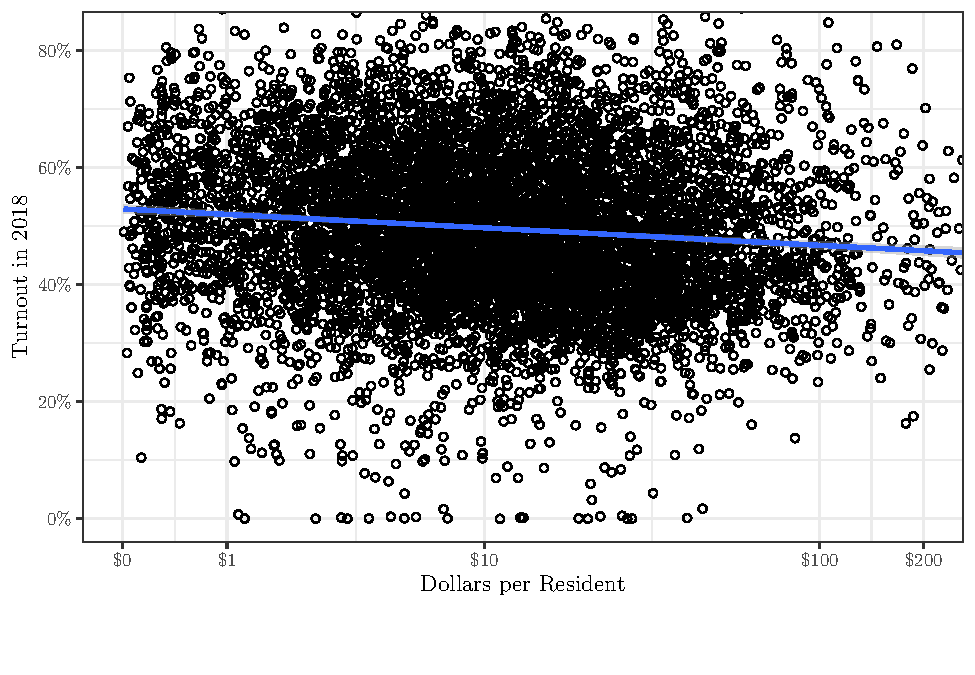
\includegraphics[height=0.4\textheight]{fees_fines_to_files/figure-latex/figures-side-1} 

}

\caption{\label{fig:to}Dollars per Resident and 2018 Turnout}\label{fig:figures-side}
\end{figure}

\begin{figure}[H]

{\centering 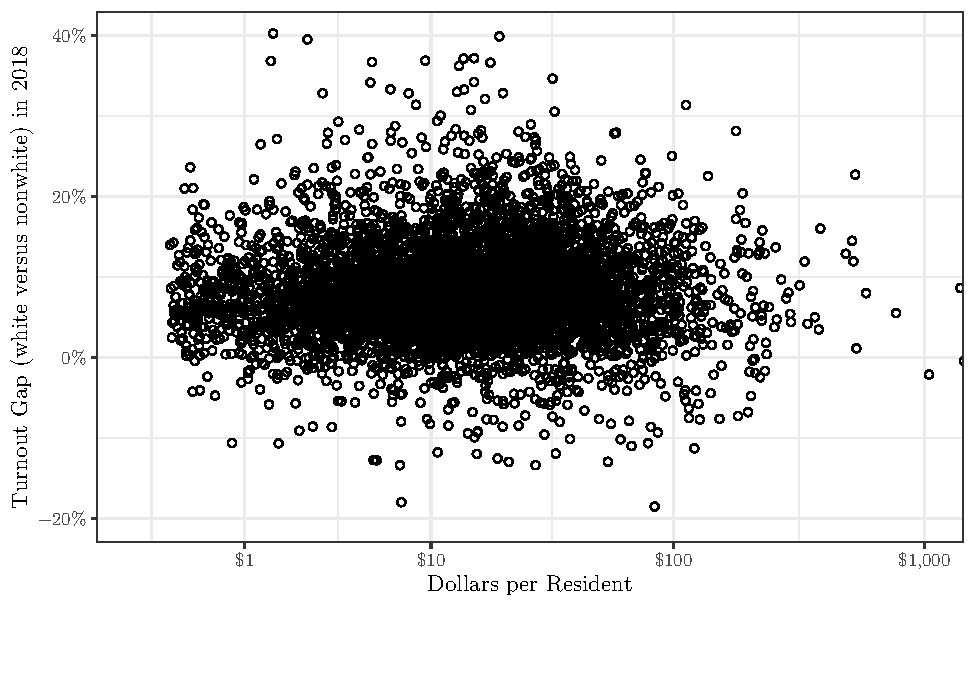
\includegraphics[height=0.4\textheight]{fees_fines_to_files/figure-latex/unnamed-chunk-1-1} 

}

\caption{\label{fig:to-gap}Dollars per Resident and 2018 Turnout Gap}\label{fig:unnamed-chunk-1}
\end{figure}

\begin{singlespace}
\input{"../temp/2wfe_reg_clean.tex"}
\end{singlespace}

\end{document}
